\documentclass[final]{beamer}
\usepackage[orientation=landscape,width=48",height=36", scale=.9]{beamerposter}
\usepackage{graphicx}	



\usepackage{booktabs} % Top and bottom rules for tables

%\usetheme{confposter}
\usepackage{exscale}
\usepackage{graphicx}  % Required for including images
\graphicspath{ {../images/} }


\usepackage {tikz}
\usetikzlibrary{arrows}
\usetikzlibrary{shapes.misc, positioning, shapes.geometric}

\newlength{\sepwid}
\newlength{\onecolwid}
\newlength{\twocolwid}
\newlength{\threecolwid}
%\setlength{\paperwidth}{48in} % A0 width: 46.8in
%\setlength{\paperheight}{36in} % A0 height: 33.1in
\setlength{\sepwid}{0.007\paperwidth} % Separation width (white space) between columns
\setlength{\onecolwid}{0.324\paperwidth} % Width of one column
\setlength{\twocolwid}{0.464\paperwidth} % Width of two columns
\setlength{\threecolwid}{0.708\paperwidth} % Width of three columns
\setlength{\topmargin}{-0.5in} % Reduce the top margin size


%\usecolortheme{beaver}
%\setbeamercolor{block body}{fg=black,bg=white} % Colors of the body of blocks
%\setbeamertemplate{navigation symbols}{}%remove navigation symbols
%\setbeamertemplate{footline}[frame number]{}

\usecaptiontemplate{
	\small
	\structure{\insertcaptionname~\insertcaptionnumber:}
	\insertcaption}

\begin{document}
	
\begin{frame}[t, noframenumbering,plain]{}

\begin{block}{\centering \Huge {An Novel LSTM RBiRNN Approach to Complex Textual Classification}}
	\begin{center}
		\Large{
			Reid McIlroy-Youn\quad MACSS \quad June 1, 2017}
	\end{center}
\end{block}


\begin{columns}[t] 
	
	%\begin{column}{\sepwid}\end{column} 
	\begin{column}{\onecolwid} 

		\begin{alertblock}{Introduction}
			Currently most analysis of scientific publications is limited to those fields available in the database used by the researches. Efforts to extend the fields usually rely on unsupervised clustering (e.g. Boyack, \textit{et al}, 2005). Presented here is a new technique for using supervised classification on scientific meta data. By using a complex model that is reading the unstructured text we can define much more abstract concepts than a similarity measure. For this analysis we looked for \textit{papers introducing new software packages, tools or interfaces}. 
		\end{alertblock}
		\begin{block}{Data}
			Our data are all articles published in the top 123 statistics journals, as identified by the Web of Science (WOS), between 2005 and 2015, giving a total of 78 971 articles. From these three journals were identified that primarily introduce new software and eight that almost never do so. These gave us 1251 positive examples and 4362 negative for training.
		\end{block}

	\begin{block}{Computation Graph}
		The neural network (NN) can be understood as a computation graph with the weights being computed via backpropagation through the graph. Figure \ref{rnn} shows the partiality unfolded graph, with the circular nodes being those learned in training. 
		\begin{figure}[!ht]
			\centering
			
			\begin{tikzpicture}[shorten >=1pt,auto,node distance=4cm, very thick]
			\node[draw, rounded corners] (1) {Abstract};
			\node[draw, rounded corners] (tokenizer) [above of=1] {Tokenizer};
			\node[draw, rounded corners] (2) [above of=tokenizer] {word2vec};
			\node[draw] (3) [above of=2] {$\vec{x}_{t}$};
			\node[draw] (4) [left of =3] {$\vec{x}_{t-1}$};
			\node[draw] (5) [right of =3] {$\vec{x}_{t+1}$};
			
			\node[draw, circle] (h1) [above of=3] {$h_t^1$};
			\node[draw, circle] (h2) [above of=4] {$h_{t-1}^1$};
			\node[draw, circle] (h3) [above of=5] {$h_{t+1}^1$};
			
			\node[draw, circle] (g1) [above of=h1] {$g_t^1$};
			\node[draw, circle] (g2) [above of=h2] {$g_{t-1}^1$};
			\node[draw, circle] (g3) [above of=h3] {$g_{t+1}^1$};
			
			\node[draw, circle] (h12) [above of=g1] {$h_t^2$};
			\node[draw, circle] (h22) [above of=g2] {$h_{t-1}^2$};
			\node[draw, circle] (h32) [above of=g3] {$h_{t+1}^2$};
			
			\node[draw, circle] (g12) [above of=h12] {$g_t^2$};
			\node[draw, circle] (g22) [above of=h22] {$g_{t-1}^2$};
			\node[draw, circle] (g32) [above of=h32] {$g_{t+1}^2$};
			
			\node[draw, regular polygon, regular polygon sides=6] (L) [above of=g12] {$\oplus$};
			
			\node[draw, rounded corners] (1t) [right = 10cm of 1]{Title};
			\node[draw, rounded corners] (tokenizert) [above of=1t] {Tokenizer};
			\node[draw, rounded corners] (2t) [above of=tokenizert] {word2vec};
			
			\node[draw] (3t) [above of=2t] {$\vec{x}_{t}$};
			\node[draw] (4t) [left of =3t] {$\vec{x}_{t-1}$};
			\node[draw] (5t) [right of =3t] {$\vec{x}_{t+1}$};
			
			\node[draw, circle] (h1t) [above of=3t] {$h^{ t}_1$};
			\node[draw, circle] (h2t) [above of=4t] {$h^{ t-1}_1$};
			\node[draw, circle] (h3t) [above of=5t] {$h^{t+1}_1$};
			
			\node[draw, circle] (g1t) [above of=h1t] {$g^{t}_1$};
			\node[draw, circle] (g2t) [above of=h2t] {$g^{t-1}_1$};
			\node[draw, circle] (g3t) [above of=h3t] {$g^{t+1}_1$};
			
			\node[draw, circle] (h1t2) [above of=g1t] {$h^{ t}_2$};
			\node[draw, circle] (h2t2) [above of=g2t] {$h^{ t-1}_2$};
			\node[draw, circle] (h3t2) [above of=g3t] {$h^{t+1}_2$};
			
			\node[draw, circle] (g1t2) [above of=h1t2] {$g^{t}_2$};
			\node[draw, circle] (g2t2) [above of=h2t2] {$g^{t-1}_2$};
			\node[draw, circle] (g3t2) [above of=h3t2] {$g^{t+1}_2$};
			
			
			\node[draw, regular polygon, regular polygon sides=6] (Lt) [above of=g1t2] {$\oplus$};
			\node[draw, circle] (u) [above right = 7.2cm of L]{$u$};
			\node[draw] (y) [above of = u]{$\hat{y}$};
			
			
			\draw[->] (L) -- (u);
			\draw[->] (Lt) -- (u);
			\draw[->] (u) -- (y);
			
			\draw[->] (1) -- (tokenizer);
			\draw[->] (tokenizer) -- (2);
			\draw[->] (2) -- (3);
			\draw[->] (2) -- (4);
			\draw[->] (2) -- (5);
			
			\draw[->] (3) -- (h1);
			\draw[->] (4) -- (h2);
			\draw[->] (5) -- (h3);
			\draw[->] (h2) -- (h1);
			\draw[->] (h1) -- (h3);
			
			\draw[->] (3)  edge[bend left] (g1);
			\draw[->] (4) edge[bend left] (g2);
			\draw[->] (5) edge[bend left] (g3);
			\draw[->] (g1) -- (g2);
			\draw[->] (g3) -- (g1);
			
			\draw[->] (h1)  edge[bend left] (h12);
			\draw[->] (h2) edge[bend left] (h22);
			\draw[->] (h3) edge[bend left] (h32);
			\draw[->] (h22) -- (h12);
			\draw[->] (h12) -- (h32);
			
			\draw[->] (g1)  edge[bend right] (g12);
			\draw[->] (g2) edge[bend right] (g22);
			\draw[->] (g3) edge[bend right] (g32);
			\draw[->] (g12) -- (g22);
			\draw[->] (g32) -- (g12);
			
			\draw[->] (g22) -- (L);
			\draw[->] (h32) -- (L);
			
			\draw[->] (1t) -- (tokenizert);
			\draw[->] (tokenizert) -- (2t);
			\draw[->] (2t) -- (3t);
			\draw[->] (2t) -- (4t);
			\draw[->] (2t) -- (5t);
			
			\draw[->] (3t) edge[bend right] (h1t);
			\draw[->] (4t) edge[bend right] (h2t);
			\draw[->] (5t) edge[bend right] (h3t);
			\draw[->] (h2t) -- (h1t);
			\draw[->] (h1t) -- (h3t);
			
			\draw[->] (3t)  edge[bend left] (g1t);
			\draw[->] (4t) edge[bend left] (g2t);
			\draw[->] (5t) edge[bend left] (g3t);
			\draw[->] (g1t) -- (g2t);
			\draw[->] (g3t) -- (g1t);
			
			\draw[->] (h1t)  edge[bend left] (h1t2);
			\draw[->] (h2t) edge[bend left] (h2t2);
			\draw[->] (h3t) edge[bend left] (h3t2);
			\draw[->] (h2t2) -- (h1t2);
			\draw[->] (h1t2) -- (h3t2);
			
			\draw[->] (g1t)  edge[bend right] (g1t2);
			\draw[->] (g2t) edge[bend right] (g2t2);
			\draw[->] (g3t) edge[bend right] (g3t2);
			\draw[->] (g1t2) -- (g2t2);
			\draw[->] (g3t2) -- (g1t2);
			
			\draw[->] (g2t2) -- (Lt);
			\draw[->] (h3t2) -- (Lt);
			\end{tikzpicture}
			\caption{Simplified recursive BiRNN layout, LSTM connections were removed for clarity. Circles are NN layers, rectangles with curved corners are the preprocessing, hexagons are combined outputs from the RNN layers, and finale output and inputs are indicated with square corners.}\label{rnn}
		\end{figure}
	\end{block}

	\end{column} 

%\begin{column}{\sepwid}\end{column} % Empty spacer column

\begin{column}{\onecolwid} % Begin a column which is two columns wide (column 2)
	\begin{alertblock}{Objectives}
		Identify new software packages in the literature
		\begin{itemize}
			\item Working with stats journals from 2005-2015
			\item Sed aliquet luctus lectus, eget aliquet leo ullamcorper consequat. Vivamus eros sem, iaculis ut euismod non, sollicitudin vel orci.
			\item Nascetur ridiculus mus.  
			\item Euismod non erat. Nam ultricies pellentesque nunc, ultrices volutpat nisl ultrices a.
		\end{itemize}
	\end{alertblock}

			

\begin{columns}[t,totalwidth=\onecolwid] % Split up the two columns wide column
	
	\begin{column}{.49\onecolwid}\vspace{-.6in} % The first column within column 2 (column 2.1)
		
		%----------------------------------------------------------------------------------------
		%	MATERIALS
		%----------------------------------------------------------------------------------------
		
		\begin{block}{Materials}
			
			\begin{figure}
				\includegraphics[width=0.49\onecolwid]{comparisonAbstract.pdf}
				\caption{Figure caption}
			\end{figure}
			
		\end{block}
		
	\end{column} % End of column 2.1
	
	\begin{column}{.49\onecolwid}\vspace{-.6in} % The second column within column 2 (column 2.2)
		\begin{block}{Figs}
			\begin{figure}
				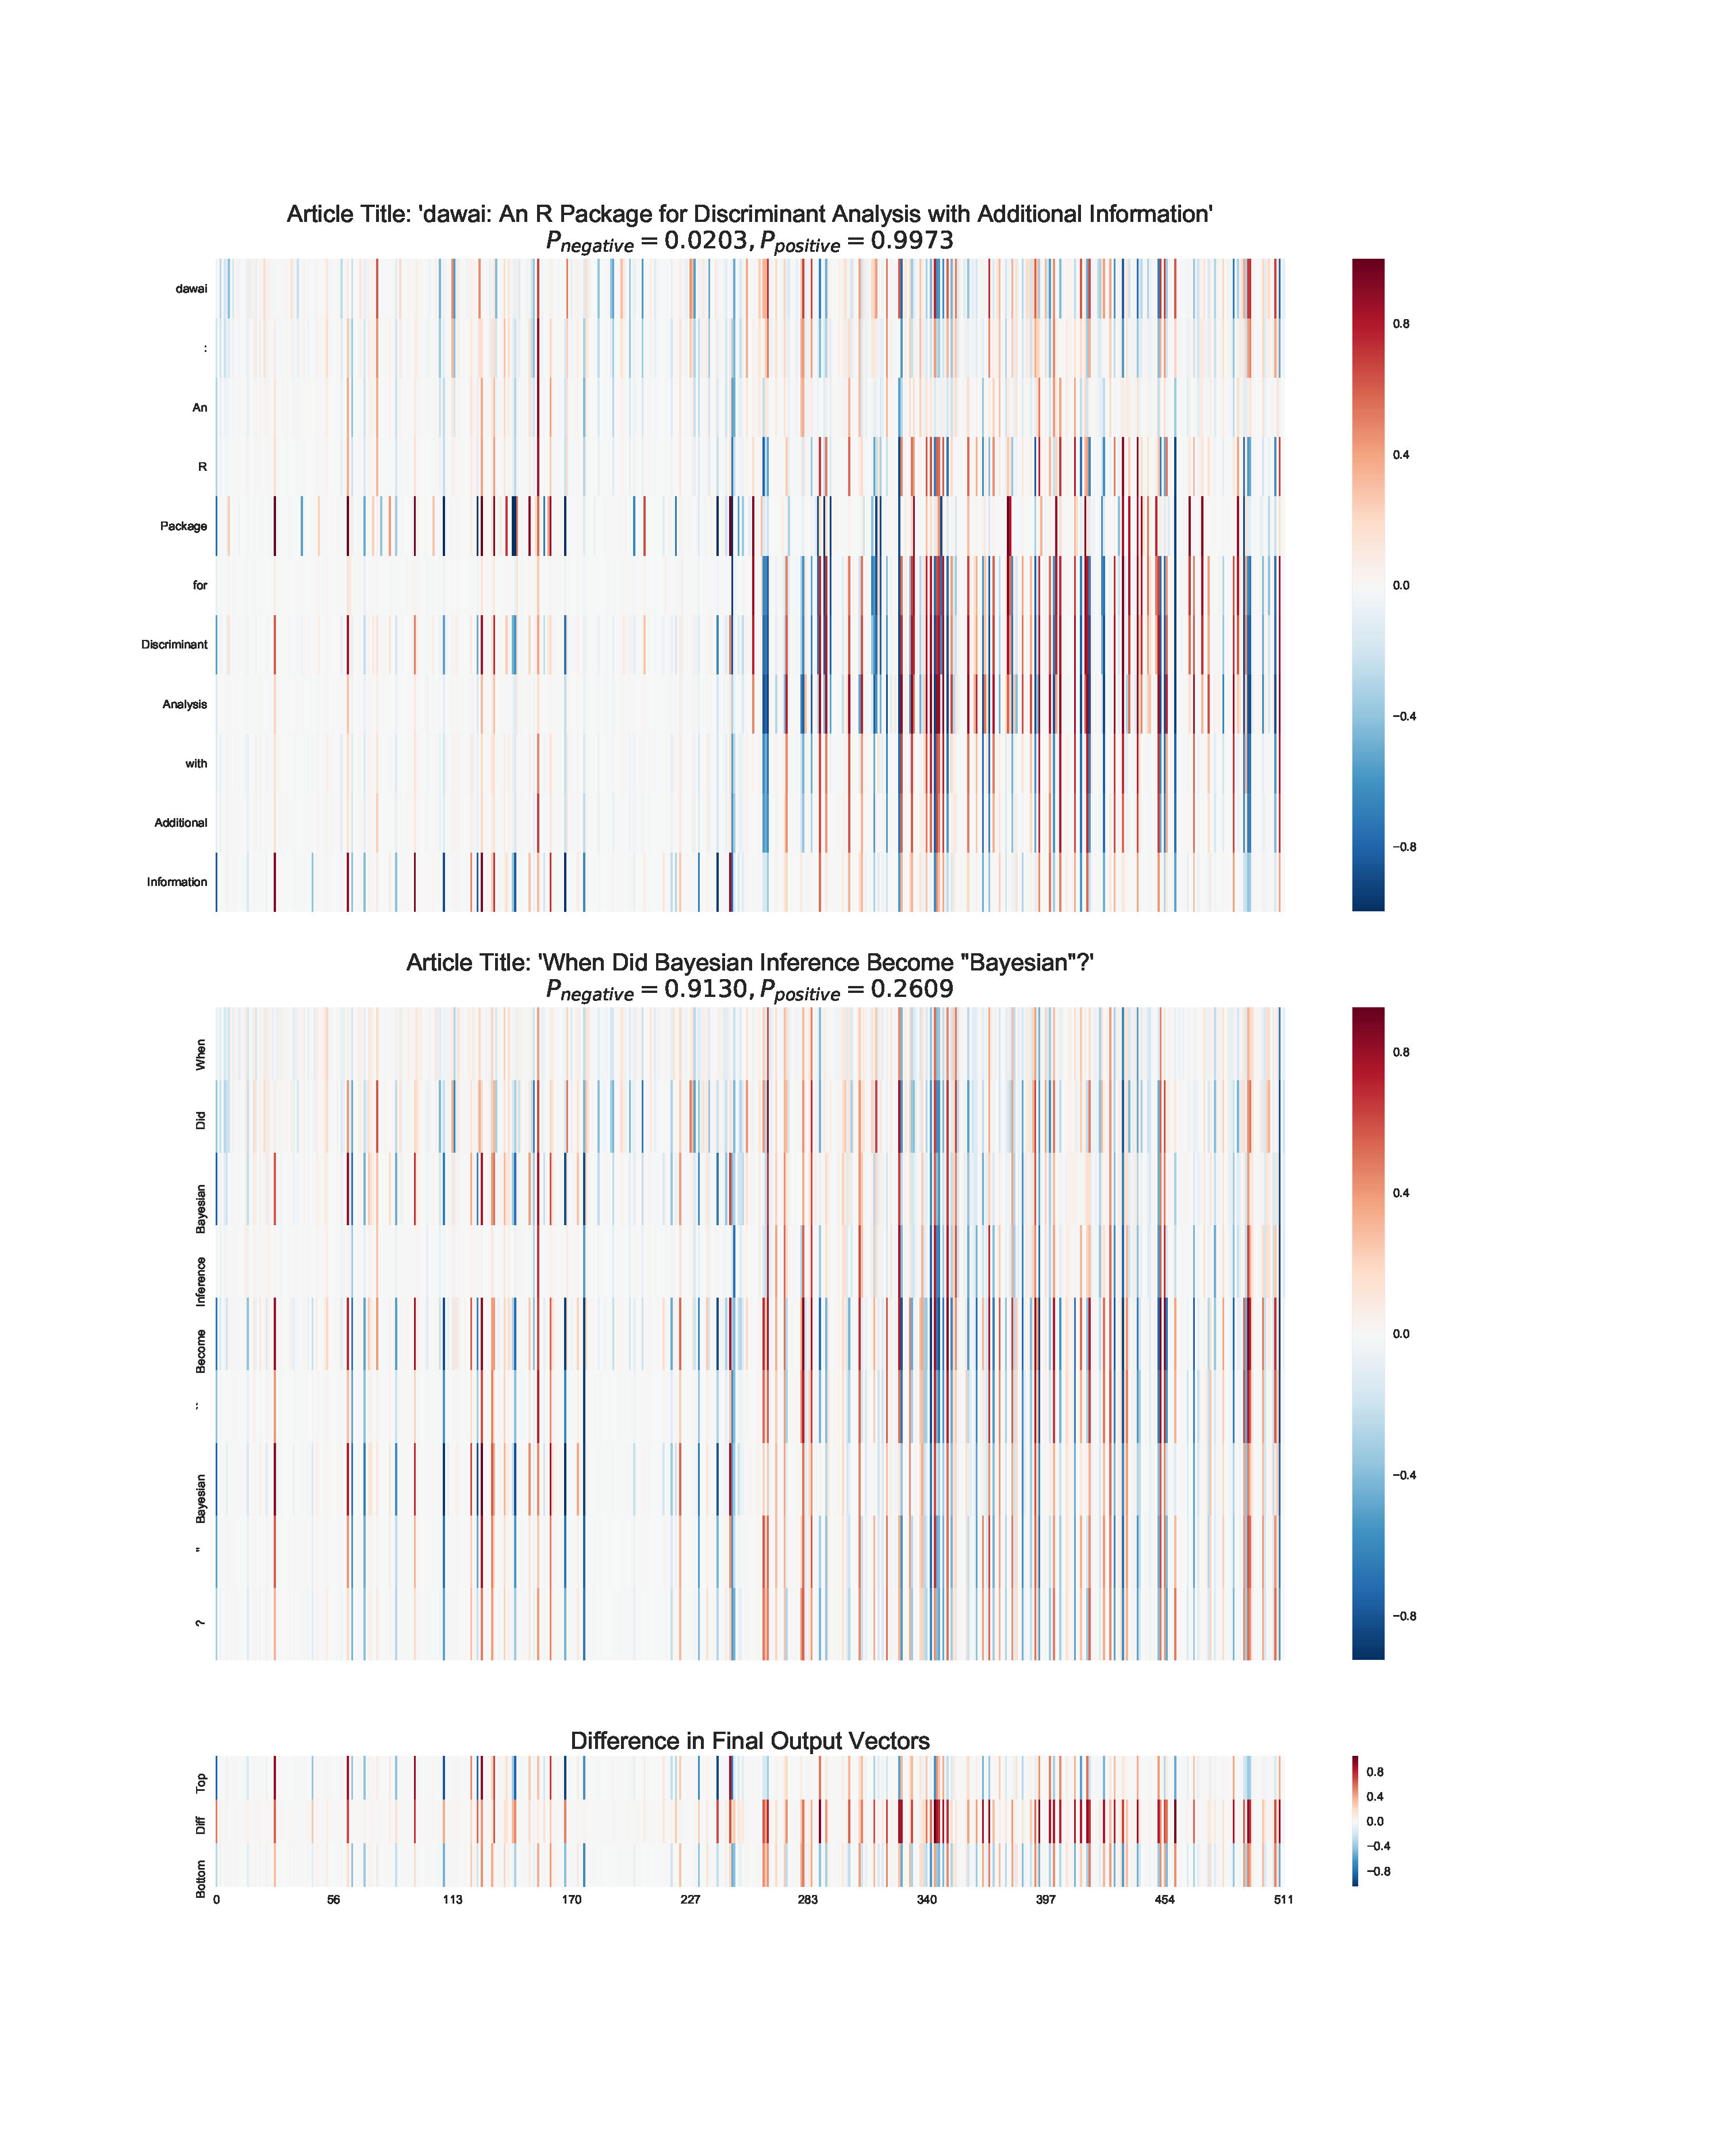
\includegraphics[width=0.49\onecolwid]{comparisonTitle.pdf}
				\caption{Figure caption}
			\end{figure}
		\end{block}
		
	\end{column} 
	
\end{columns}

\end{column} 


\begin{column}{\onecolwid} % The third column
	\begin{block}{Model Statistics}
		\begin{table}
			\vspace{2ex}
			\begin{tabular}{|l c|}
				\toprule
				\textbf{Treatments} & \textbf{Response 1} \\
				\midrule
				Epochs & 9  \\
				Batches per Epoch & 500\\
				Testing Loss &  0.115 \\
				Testing Error Rate & 0.040 \\
				Detection Rate & 0.973\\
				False Positive Rate& 0.043\\
				\bottomrule
			\end{tabular}
			\caption{Table caption}
		\end{table}
		
	\end{block}
\begin{block}{Results}
	\begin{table}
		\vspace{2ex}
		\begin{tabular}{|l c|}
			\toprule
			\textbf{Treatments} & \textbf{Response 1} \\
			\midrule
			Epochs & 9  \\
			Batches per Epoch & 500\\
			Testing Loss &  0.115 \\
			Testing Error Rate & 0.040 \\
			Detection Rate & 0.973\\
			False Positive Rate& 0.043\\
			\bottomrule
		\end{tabular}
		\caption{Table caption}
	\end{table}
	
\end{block}
\begin{block}{Counts}
	\begin{figure}
		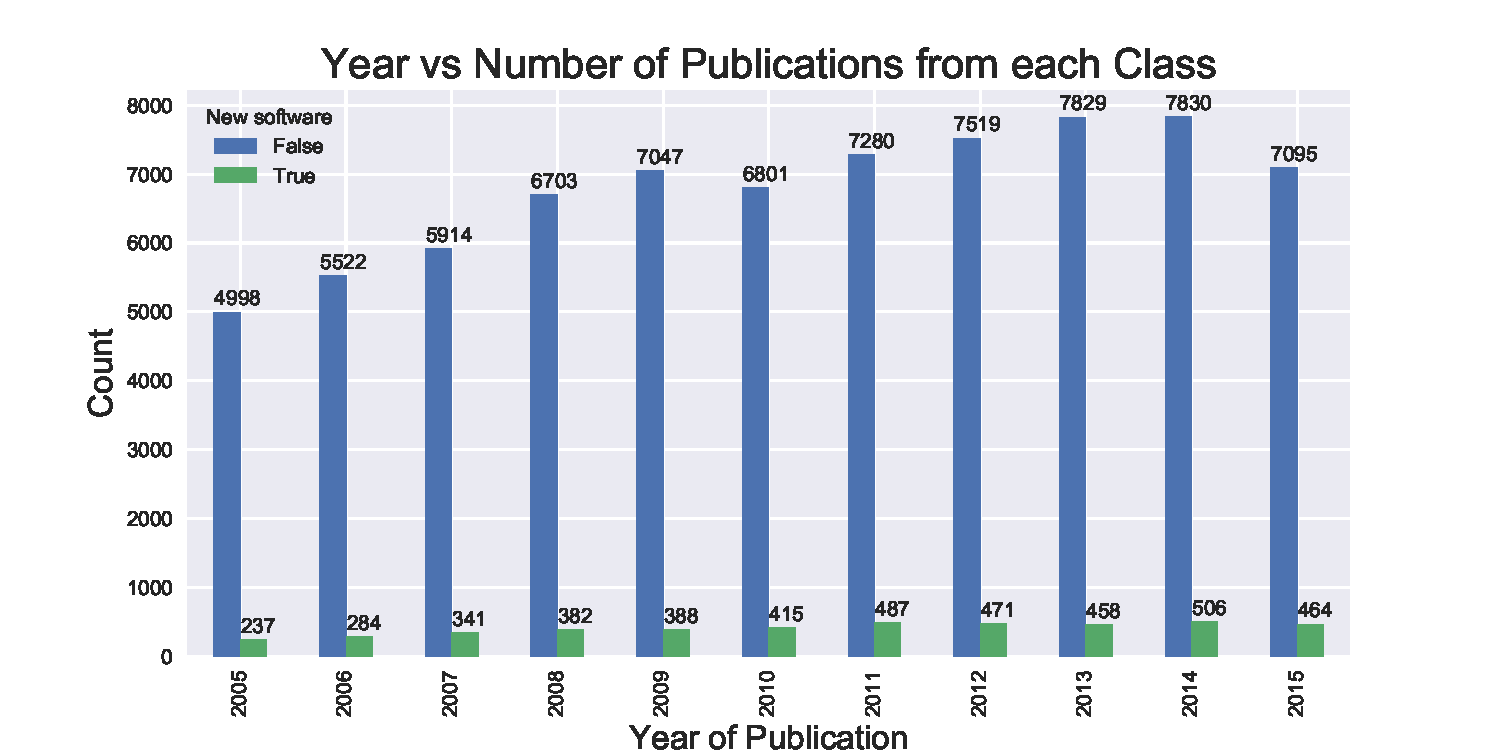
\includegraphics[width=0.8\linewidth]{countvyear.pdf}
		\caption{Figure caption}
	\end{figure}
\begin{figure}
	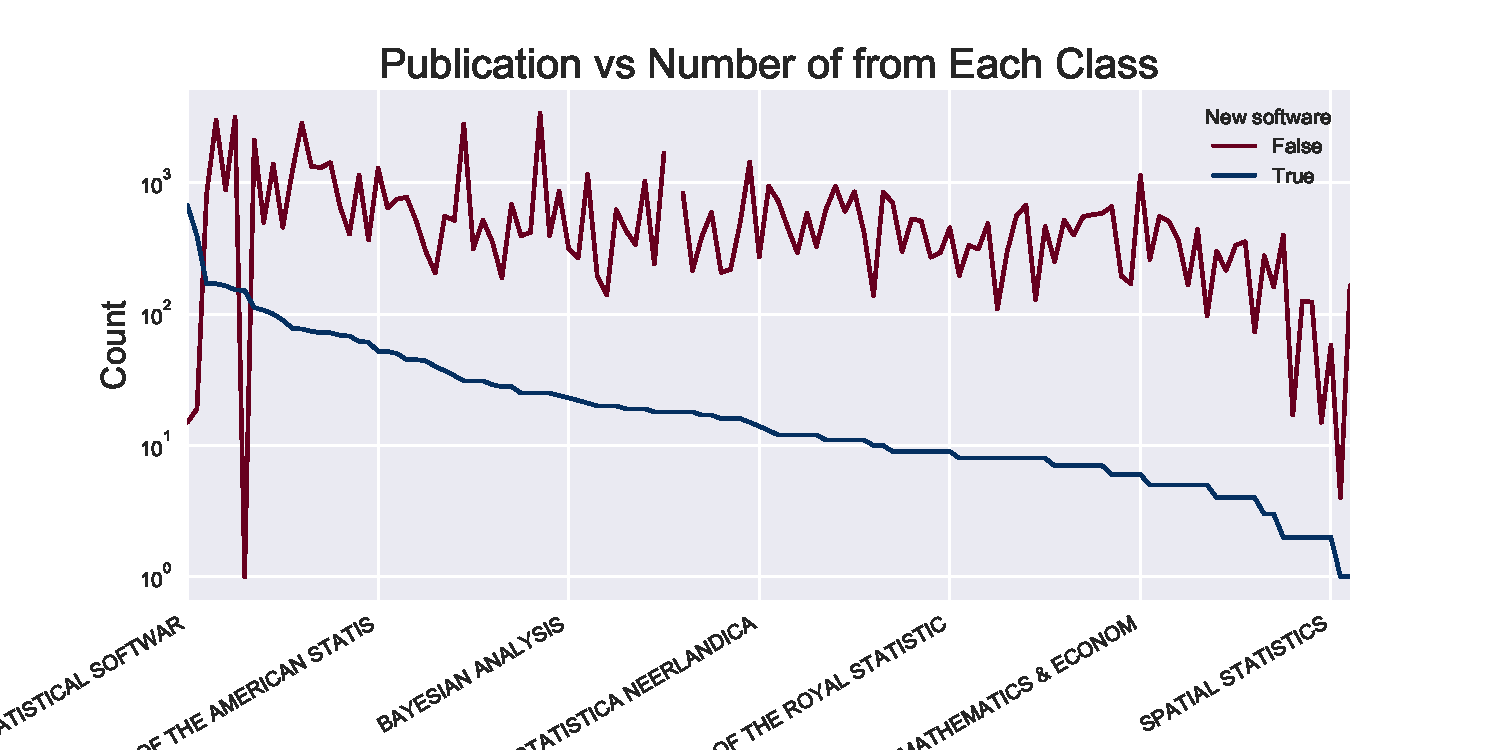
\includegraphics[width=0.8\linewidth]{countvpub.pdf}
	\caption{Figure caption}
\end{figure}

\end{block}
\end{column} % End of the third column
%\begin{column}{\sepwid}\end{column} % Empty spacer column
\end{columns}

\end{frame}

\end{document}